% Options for packages loaded elsewhere
% Options for packages loaded elsewhere
\PassOptionsToPackage{unicode}{hyperref}
\PassOptionsToPackage{hyphens}{url}
%
\documentclass[
  14pt,
  ignorenonframetext,
  aspectratio=169,
]{beamer}
\newif\ifbibliography
\usepackage{pgfpages}
\setbeamertemplate{caption}[numbered]
\setbeamertemplate{caption label separator}{: }
\setbeamercolor{caption name}{fg=normal text.fg}
\beamertemplatenavigationsymbolsempty
% remove section numbering
\setbeamertemplate{part page}{
  \centering
  \begin{beamercolorbox}[sep=16pt,center]{part title}
    \usebeamerfont{part title}\insertpart\par
  \end{beamercolorbox}
}
\setbeamertemplate{section page}{
  \centering
  \begin{beamercolorbox}[sep=12pt,center]{section title}
    \usebeamerfont{section title}\insertsection\par
  \end{beamercolorbox}
}
\setbeamertemplate{subsection page}{
  \centering
  \begin{beamercolorbox}[sep=8pt,center]{subsection title}
    \usebeamerfont{subsection title}\insertsubsection\par
  \end{beamercolorbox}
}
% Prevent slide breaks in the middle of a paragraph
\widowpenalties 1 10000
\raggedbottom
\usepackage{iftex}
\ifPDFTeX
  \usepackage[T1]{fontenc}
  \usepackage[utf8]{inputenc}
  \usepackage{textcomp} % provide euro and other symbols
\else % if luatex or xetex
  \usepackage{unicode-math} % this also loads fontspec
  \defaultfontfeatures{Scale=MatchLowercase}
  \defaultfontfeatures[\rmfamily]{Ligatures=TeX,Scale=1}
\fi
\usepackage{lmodern}

\usetheme[]{monash}
\ifPDFTeX\else
  % xetex/luatex font selection
\fi
% Use upquote if available, for straight quotes in verbatim environments
\IfFileExists{upquote.sty}{\usepackage{upquote}}{}
\IfFileExists{microtype.sty}{% use microtype if available
  \usepackage[]{microtype}
  \UseMicrotypeSet[protrusion]{basicmath} % disable protrusion for tt fonts
}{}
\makeatletter
\@ifundefined{KOMAClassName}{% if non-KOMA class
  \IfFileExists{parskip.sty}{%
    \usepackage{parskip}
  }{% else
    \setlength{\parindent}{0pt}
    \setlength{\parskip}{6pt plus 2pt minus 1pt}}
}{% if KOMA class
  \KOMAoptions{parskip=half}}
\makeatother

\usepackage{color}
\usepackage{fancyvrb}
\newcommand{\VerbBar}{|}
\newcommand{\VERB}{\Verb[commandchars=\\\{\}]}
\DefineVerbatimEnvironment{Highlighting}{Verbatim}{commandchars=\\\{\}}
% Add ',fontsize=\small' for more characters per line
\usepackage{framed}
\definecolor{shadecolor}{RGB}{248,248,248}
\newenvironment{Shaded}{\begin{snugshade}}{\end{snugshade}}
\newcommand{\AlertTok}[1]{\textcolor[rgb]{0.94,0.16,0.16}{#1}}
\newcommand{\AnnotationTok}[1]{\textcolor[rgb]{0.56,0.35,0.01}{\textbf{\textit{#1}}}}
\newcommand{\AttributeTok}[1]{\textcolor[rgb]{0.13,0.29,0.53}{#1}}
\newcommand{\BaseNTok}[1]{\textcolor[rgb]{0.00,0.00,0.81}{#1}}
\newcommand{\BuiltInTok}[1]{#1}
\newcommand{\CharTok}[1]{\textcolor[rgb]{0.31,0.60,0.02}{#1}}
\newcommand{\CommentTok}[1]{\textcolor[rgb]{0.56,0.35,0.01}{\textit{#1}}}
\newcommand{\CommentVarTok}[1]{\textcolor[rgb]{0.56,0.35,0.01}{\textbf{\textit{#1}}}}
\newcommand{\ConstantTok}[1]{\textcolor[rgb]{0.56,0.35,0.01}{#1}}
\newcommand{\ControlFlowTok}[1]{\textcolor[rgb]{0.13,0.29,0.53}{\textbf{#1}}}
\newcommand{\DataTypeTok}[1]{\textcolor[rgb]{0.13,0.29,0.53}{#1}}
\newcommand{\DecValTok}[1]{\textcolor[rgb]{0.00,0.00,0.81}{#1}}
\newcommand{\DocumentationTok}[1]{\textcolor[rgb]{0.56,0.35,0.01}{\textbf{\textit{#1}}}}
\newcommand{\ErrorTok}[1]{\textcolor[rgb]{0.64,0.00,0.00}{\textbf{#1}}}
\newcommand{\ExtensionTok}[1]{#1}
\newcommand{\FloatTok}[1]{\textcolor[rgb]{0.00,0.00,0.81}{#1}}
\newcommand{\FunctionTok}[1]{\textcolor[rgb]{0.13,0.29,0.53}{\textbf{#1}}}
\newcommand{\ImportTok}[1]{#1}
\newcommand{\InformationTok}[1]{\textcolor[rgb]{0.56,0.35,0.01}{\textbf{\textit{#1}}}}
\newcommand{\KeywordTok}[1]{\textcolor[rgb]{0.13,0.29,0.53}{\textbf{#1}}}
\newcommand{\NormalTok}[1]{#1}
\newcommand{\OperatorTok}[1]{\textcolor[rgb]{0.81,0.36,0.00}{\textbf{#1}}}
\newcommand{\OtherTok}[1]{\textcolor[rgb]{0.56,0.35,0.01}{#1}}
\newcommand{\PreprocessorTok}[1]{\textcolor[rgb]{0.56,0.35,0.01}{\textit{#1}}}
\newcommand{\RegionMarkerTok}[1]{#1}
\newcommand{\SpecialCharTok}[1]{\textcolor[rgb]{0.81,0.36,0.00}{\textbf{#1}}}
\newcommand{\SpecialStringTok}[1]{\textcolor[rgb]{0.31,0.60,0.02}{#1}}
\newcommand{\StringTok}[1]{\textcolor[rgb]{0.31,0.60,0.02}{#1}}
\newcommand{\VariableTok}[1]{\textcolor[rgb]{0.00,0.00,0.00}{#1}}
\newcommand{\VerbatimStringTok}[1]{\textcolor[rgb]{0.31,0.60,0.02}{#1}}
\newcommand{\WarningTok}[1]{\textcolor[rgb]{0.56,0.35,0.01}{\textbf{\textit{#1}}}}

\usepackage{longtable,booktabs,array}
\newcounter{none} % for unnumbered tables
\usepackage{calc} % for calculating minipage widths
\usepackage{caption}
% Make caption package work with longtable
\makeatletter
\def\fnum@table{\tablename~\thetable}
\makeatother
\usepackage{graphicx}
\makeatletter
\newsavebox\pandoc@box
\newcommand*\pandocbounded[1]{% scales image to fit in text height/width
  \sbox\pandoc@box{#1}%
  \Gscale@div\@tempa{\textheight}{\dimexpr\ht\pandoc@box+\dp\pandoc@box\relax}%
  \Gscale@div\@tempb{\linewidth}{\wd\pandoc@box}%
  \ifdim\@tempb\p@<\@tempa\p@\let\@tempa\@tempb\fi% select the smaller of both
  \ifdim\@tempa\p@<\p@\scalebox{\@tempa}{\usebox\pandoc@box}%
  \else\usebox{\pandoc@box}%
  \fi%
}
% Set default figure placement to htbp
\def\fps@figure{htbp}
\makeatother





\setlength{\emergencystretch}{3em} % prevent overfull lines

\providecommand{\tightlist}{%
  \setlength{\itemsep}{0pt}\setlength{\parskip}{0pt}}



 


% Colors
\definecolor{shadecolor}{RGB}{225,225,225}
\setbeamercolor{description item}{fg=Orange}
\definecolor{MonashBlue}{RGB}{66,109,152}
\definecolor{burntorange}{rgb}{0.8, 0.33, 0.0}

% Packages
\usepackage{amsmath, bm, amssymb, amsthm, mathrsfs,pifont}
\usepackage{url}
\usepackage{multirow, booktabs, float, textcmds, siunitx}
\usepackage{bm,booktabs,animate,ragged2e,multicol,microtype,hyperref}
\usepackage{fontawesome5}

% Figures
\graphicspath{{figs/}}

% Fonts
\fontsize{13}{15}\sf
\setbeamerfont{title}{series=\bfseries,parent=structure,size=\fontsize{24}{24}}
\ifcsname Shaded\endcsname
  \definecolor{shadecolor}{RGB}{225,225,225}
  \renewenvironment{Shaded}{\vspace*{0.15cm}\color{black}\fontsize{10}{10}\sf\begin{snugshade}\color{black}}{\end{snugshade}}
\fi

% gt dependencies
\usepackage{longtable,caption,setspace}
\captionsetup{font={small,stretch=0.80}}

% My definitions

\def\E{\text{E}}
\def\V{\text{Var}}
\def\up#1{\raisebox{-0.3cm}{#1}}
\def\pred#1#2#3{\hat{#1}_{#2|#3}}
\def\damped{$_\text{d}$}
\def\h+{h_{m}^{+}}
\def\str#1{\rlap{#1}\textcolor{red}{\rule{1cm}{0.1cm}}}

\def\st#1{\rlap{#1}\textcolor{red}{\rule{1cm}{0.1cm}}}
\def\bY{\bm{y}}
\def\by{\bm{y}}
\def\bS{\bm{S}}
\def\bI{\text{\rm\textbf{I}}}
\def\bbeta{\bm{\beta}}
\def\bSigma{\bm{\Sigma}}
\def\bW{\bm{\Sigma}}
\def\Var{\text{Var}}
\def\var{\text{Var}}
\def\bOmega{\bm{\Omega}}
\def\bLambda{\bm{\Lambda}}
\let\mc\multicolumn
\def\hl{\color[RGB]{230, 172, 0}}

\def\forecast{\begin{alertblock}{}\fontsize{10}{11}\sf
 A forecast is an estimate of the probability distribution of a variable to be observed in the future.
\end{alertblock}}

\def\simfutures{\begin{textblock}{2.9}(12.8,7.7)
\begin{block}{}\fontsize{10}{11}\sf
Simulated futures from an ETS model
\end{block}\end{textblock}}

\setbeamertemplate{title page}
{\placefig{0}{-0.5}{width=1.01\paperwidth,height=1.45\paperheight}{africa1.jpg}
\begin{textblock}{8.5}(.5,0.2)
  \raggedright\fontsize{20}{20}\selectfont\bfseries\sffamily\textcolor{white}{\inserttitle}\\[0.2cm]
  \fontsize{12}{12}\selectfont\bfseries\sffamily\textcolor{white}{\insertsubtitle}
  \end{textblock}
\placefig{.5}{6.2}{width=2.4cm}{tsibble.png}
\placefig{2.9}{6.2}{width=2.4cm}{feasts.png}
\placefig{5.3}{6.2}{width=2.4cm}{fable.png}
\begin{textblock}{7.5}(10.6,-.1)
  {\fontsize{9}{9}\sf\color{white}https://workshop.f4sg.org/africast/}
\end{textblock}
}

% Tikz plots
\usepackage{tikz}
\usetikzlibrary{trees,shapes,arrows,matrix,shadows,positioning,calc}
\tikzstyle{decision} = [diamond, draw, fill=blue!20,
    text width=4.5em, text badly centered, node distance=4cm, inner sep=0pt]
\tikzstyle{block} = [rectangle, draw, fill=blue!20,
    text width=5cm, text centered, rounded corners, minimum height=4em]
\tikzstyle{line} = [draw, thick, -latex']
\tikzstyle{cloud} = [draw, ellipse,fill=red!20, node distance=3cm,
    minimum height=2em, text centered]
\tikzstyle{connector} = [->,thick]

\tikzset{
  basic/.style  = {draw, text width=2cm, font=\sffamily, rectangle},
  root/.style   = {basic, text width=3cm, rounded corners=2pt, thin, align=center, fill=red!30},
  level 2a/.style = {basic, rounded corners=2pt, thin,align=center, fill=blue!50, text width=7em},
  level 2b/.style = {basic, rounded corners=2pt, thin,align=center, fill=green!50, text width=7em},
  level 3a/.style = {basic, rounded corners=2pt, thin, align=center, fill=blue!30, text width=4em},
  level 3b/.style = {basic, rounded corners=2pt, thin, align=center, fill=green!30, text width=4em},
  level 4a/.style = {basic, rounded corners=2pt, thin, align=left, fill=blue!10, text width=3.5em},
  level 4b/.style = {basic, rounded corners=2pt, thin, align=left, fill=green!10, text width=3.5em}
}

% % BIBLIOGRAPHIES
% \usepackage[style=authoryear,bibencoding=utf8,minnames=1,maxnames=4, maxbibnames=99,natbib=true,dashed=false,terseinits=true,giveninits=true,uniquename=false,uniquelist=false,labeldate=true,doi=false, isbn=false, natbib=true,backend=biber]{biblatex}

% \DeclareFieldFormat{url}{\url{#1}}
% \DeclareFieldFormat[article]{pages}{#1}
% \DeclareFieldFormat[inproceedings]{pages}{\lowercase{pp.}#1}
% \DeclareFieldFormat[incollection]{pages}{\lowercase{pp.}#1}
% \DeclareFieldFormat[article]{volume}{\mkbibbold{#1}}
% \DeclareFieldFormat[article]{number}{\mkbibparens{#1}}
% \DeclareFieldFormat[article]{title}{\MakeCapital{#1}}
% \DeclareFieldFormat[article]{url}{}
% \DeclareFieldFormat[Techreport]{Url}{}
% \DeclareFieldFormat[book]{url}{}
% \DeclareFieldFormat[inbook]{url}{}
% \DeclareFieldFormat[incollection]{url}{}
% \DeclareFieldFormat[inproceedings]{url}{}
% \DeclareFieldFormat[inproceedings]{title}{#1}
% \DeclareFieldFormat{shorthandwidth}{#1}
% %\DeclareFieldFormat{extrayear}{}
% % No dot before number of articles
% \usepackage{xpatch}
% \xpatchbibmacro{volume+number+eid}{\setunit*{\adddot}}{}{}{}
% % Remove In: for an article.
% \renewbibmacro{in:}{%
%   \ifentrytype{article}{}{%
%   \printtext{\bibstring{in}\intitlepunct}}}

% \AtEveryBibitem{\clearfield{month}}
% \AtEveryCitekey{\clearfield{month}}
% \AtBeginBibliography{\fontsize{11}{11}\sf}
\setbeamertemplate{frametitle continuation}{}
\makeatletter
\@ifpackageloaded{caption}{}{\usepackage{caption}}
\AtBeginDocument{%
\ifdefined\contentsname
  \renewcommand*\contentsname{Table of contents}
\else
  \newcommand\contentsname{Table of contents}
\fi
\ifdefined\listfigurename
  \renewcommand*\listfigurename{List of Figures}
\else
  \newcommand\listfigurename{List of Figures}
\fi
\ifdefined\listtablename
  \renewcommand*\listtablename{List of Tables}
\else
  \newcommand\listtablename{List of Tables}
\fi
\ifdefined\figurename
  \renewcommand*\figurename{Figure}
\else
  \newcommand\figurename{Figure}
\fi
\ifdefined\tablename
  \renewcommand*\tablename{Table}
\else
  \newcommand\tablename{Table}
\fi
}
\@ifpackageloaded{float}{}{\usepackage{float}}
\floatstyle{ruled}
\@ifundefined{c@chapter}{\newfloat{codelisting}{h}{lop}}{\newfloat{codelisting}{h}{lop}[chapter]}
\floatname{codelisting}{Listing}
\newcommand*\listoflistings{\listof{codelisting}{List of Listings}}
\makeatother
\makeatletter
\makeatother
\makeatletter
\@ifpackageloaded{caption}{}{\usepackage{caption}}
\@ifpackageloaded{subcaption}{}{\usepackage{subcaption}}
\makeatother

\usepackage{bookmark}
\IfFileExists{xurl.sty}{\usepackage{xurl}}{} % add URL line breaks if available
\urlstyle{same}
% fallback for those not using the hyperref driver hyperxmp:
\makeatletter
\@ifundefined{xmpquote}{\newcommand{\xmpquote}[1]{#1}}{}
\makeatother
\hypersetup{
  pdftitle={Africast-Time Series Analysis \& Forecasting Using R},
  hidelinks,
  pdfcreator={LaTeX via pandoc}}


\title{\texorpdfstring{Africast-Time Series Analysis \& Forecasting
Using R}{Africast-Time Series Analysis \& Forecasting Using R}}
\subtitle{\texorpdfstring{1. Basics of time series and data
structures}{1. Basics of time series and data structures}}
\author{}
\date{5 October 2026}

\begin{document}
\frame{\titlepage}


\begin{frame}{Outline}
\protect\phantomsection\label{outline}
\vspace*{0.7cm}\tableofcontents
\end{frame}

\section{Introduction to forecasting}\label{introduction-to-forecasting}

\begin{frame}{What is a forecast?}
\protect\phantomsection\label{what-is-a-forecast}
\fontsize{12}{13}\sf

Estimating how a sequence of observations will continue into the future,
using all information available now.

\begin{center}
\includegraphics[width=0.9\linewidth,height=\textheight,keepaspectratio]{01_basics_data_structure_files/figure-beamer/forecasting-1.pdf}
\end{center}
\end{frame}

\begin{frame}{What data do we need?}
\protect\phantomsection\label{what-data-do-we-need}
\begin{enumerate}
\tightlist
\item
  Historical data on the variable to forecast
\item
  Past and future values of predictors

  \begin{itemize}
  \tightlist
  \item
    Deterministic (e.g.~holidays)
  \item
    Stochastic (e.g.~temperature)
  \end{itemize}
\item
  Expert knowledge and context

  \begin{itemize}
  \tightlist
  \item
    New information
  \end{itemize}
\end{enumerate}
\end{frame}

\begin{frame}{Why forecast?}
\protect\phantomsection\label{why-forecast}
Why do you use forecasts?

\pause

\fontsize{12}{13}\sf

{\def\LTcaptype{none} % do not increment counter
\begin{longtable}[]{@{}lc@{}}
\toprule\noalign{}
Decision & Forecast \\
\midrule\noalign{}
\endhead
Build a new hospital in the next 10 years? & ? \\
Call centre staff needed next week? & ? \\
Vaccine doses needed next month? & ? \\
\bottomrule\noalign{}
\end{longtable}
}

\begin{itemize}
\tightlist
\item
  Supports planning
\item
  Informs decisions
\item
  Provides evidence
\end{itemize}
\end{frame}

\begin{frame}{Forecasting workflow}
\protect\phantomsection\label{forecasting-workflow}
\begin{center}
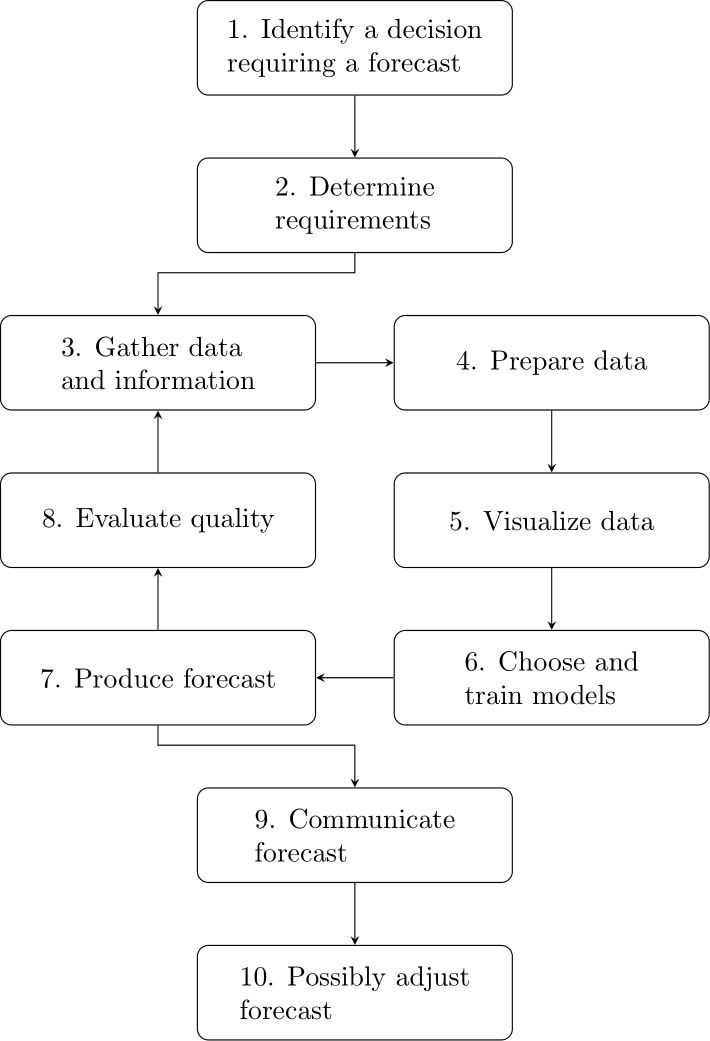
\includegraphics[width=0.32\linewidth,height=\textheight,keepaspectratio]{figs/forecasting_workflow.png}
\end{center}
\end{frame}

\begin{frame}{Packages for this course}
\protect\phantomsection\label{packages-for-this-course}
\begin{textblock}{4.2}(10.8,0.3)\begin{alertblock}{}\Large\textbf{tidyverts.org}\end{alertblock}\end{textblock}

\placefig{1.8}{1.3}{width=3cm}{tsibble.png}
\placefig{5.2}{1.3}{width=3cm}{mixtime.png}
\placefig{8.6}{1.3}{width=3cm}{tsibbledata.png}
\placefig{3.5}{4.6}{width=3cm}{feasts.png}
\placefig{6.9}{4.6}{width=3cm}{ggtime.png}
\placefig{10.3}{4.6}{width=3cm}{fable.png}
\end{frame}

\begin{frame}[fragile]{Packages for this course}
\protect\phantomsection\label{packages-for-this-course-1}
\fontsize{11}{12}\sf

\begin{Shaded}
\begin{Highlighting}[]
\CommentTok{\# Data, graphics and forecasting}
\FunctionTok{library}\NormalTok{(fpp3)}
\end{Highlighting}
\end{Shaded}

\begin{verbatim}
-- Attaching packages ------------------------------ fpp3 1.0.3 --
\end{verbatim}

\begin{verbatim}
v tibble      3.3.1          v tsibble     1.2.0.9000
v dplyr       1.2.1          v tsibbledata 0.4.1     
v tidyr       1.3.2          v ggtime      0.2.0.9000
v lubridate   1.9.5          v feasts      0.5.0     
v ggplot2     4.0.3          v fable       0.5.0.9000
\end{verbatim}

\pause

\begin{Shaded}
\begin{Highlighting}[]
\CommentTok{\# Time classes for the index (load after fpp3)}
\FunctionTok{library}\NormalTok{(mixtime)}
\end{Highlighting}
\end{Shaded}
\end{frame}

\section{Time series data}\label{time-series-data}

\begin{frame}{Time series data}
\protect\phantomsection\label{time-series-data-1}
\begin{itemize}
\tightlist
\item
  Four-yearly Olympic winning times
\item
  Annual Google profits
\item
  Quarterly Australian beer production
\item
  Monthly rainfall
\item
  Weekly retail sales
\item
  Daily IBM stock prices
\item
  Hourly electricity demand
\item
  5-minute freeway traffic counts
\item
  Time-stamped stock transaction data
\end{itemize}
\end{frame}

\begin{frame}{Your time series}
\protect\phantomsection\label{your-time-series}
\begin{block}{}\Large
What time series do you work with?
\end{block}

\pause

\begin{itemize}
\tightlist
\item
  What is measured?
\item
  How often?
\item
  One series, or many?
\end{itemize}
\end{frame}

\begin{frame}{What makes it a time series?}
\protect\phantomsection\label{what-makes-it-a-time-series}
\begin{block}{}
Observations + \alert{when} they happened.
\end{block}

\begin{itemize}
\tightlist
\item
  The time column is the \alert{index}
\item
  Observations are ordered in time
\item
  The frequency matters
\end{itemize}
\end{frame}

\section{tsibble objects}\label{tsibble-objects}

\begin{frame}{A \texttt{tsibble} has three parts}
\protect\phantomsection\label{a-tsibble-has-three-parts}
\begin{block}{}
A \alert{tsibble} stores one or more time series in a table.
\end{block}

\begin{itemize}
\tightlist
\item
  \textbf{Index}: when
\item
  \textbf{Key}: which series (optional)
\item
  \textbf{Measures}: what was observed
\end{itemize}

\vspace*{0.3cm}

Works with tidyverse functions.
\end{frame}

\begin{frame}[fragile]{\texttt{tsibble} objects}
\protect\phantomsection\label{tsibble-objects-1}
\fontsize{10}{11.2}\sf

\begin{Shaded}
\begin{Highlighting}[]
\NormalTok{global\_economy}
\end{Highlighting}
\end{Shaded}

\begin{verbatim}
# A tsibble: 15,150 x 6 [1Y]
# Key:       Country [263]
    Year Country             GDP Imports Exports Population
   <dbl> <fct>             <dbl>   <dbl>   <dbl>      <dbl>
 1  1960 Afghanistan  537777811.    7.02    4.13    8996351
 2  1961 Afghanistan  548888896.    8.10    4.45    9166764
 3  1962 Afghanistan  546666678.    9.35    4.88    9345868
 4  1963 Afghanistan  751111191.   16.9     9.17    9533954
 5  1964 Afghanistan  800000044.   18.1     8.89    9731361
 6  1965 Afghanistan 1006666638.   21.4    11.3     9938414
 7  1966 Afghanistan 1399999967.   18.6     8.57   10152331
 8  1967 Afghanistan 1673333418.   14.2     6.77   10372630
 9  1968 Afghanistan 1373333367.   15.2     8.90   10604346
10  1969 Afghanistan 1408888922.   15.0    10.1    10854428
# i 15,140 more rows
\end{verbatim}

\only<2->{\begin{textblock}{1.05}(1.5,3.2)
\begin{alertblock}{}\fontsize{10}{10}\sf\mbox{Index}\phantom{dg}\end{alertblock}
\end{textblock}}
\only<3->{\begin{textblock}{1.6}(2.72,3.2)
\begin{alertblock}{}\fontsize{10}{10}\sf Key\phantom{dg}\end{alertblock}
\end{textblock}}
\only<4>{\begin{textblock}{6.3}(5.2,3.2)
\begin{alertblock}{}\fontsize{10}{10}\sf Measures\phantom{dg}\end{alertblock}
\end{textblock}}
\end{frame}

\begin{frame}[fragile]{\texttt{tsibble} objects}
\protect\phantomsection\label{tsibble-objects-2}
\fontsize{10}{11.2}\sf

\begin{Shaded}
\begin{Highlighting}[]
\NormalTok{tourism}
\end{Highlighting}
\end{Shaded}

\begin{verbatim}
# A tsibble: 24,320 x 5 [1Q]
# Key:       Region, State, Purpose [304]
   Quarter Region   State Purpose  Trips
     <qtr> <chr>    <chr> <chr>    <dbl>
 1 1998 Q1 Adelaide SA    Business  135.
 2 1998 Q2 Adelaide SA    Business  110.
 3 1998 Q3 Adelaide SA    Business  166.
 4 1998 Q4 Adelaide SA    Business  127.
 5 1999 Q1 Adelaide SA    Business  137.
 6 1999 Q2 Adelaide SA    Business  200.
 7 1999 Q3 Adelaide SA    Business  169.
 8 1999 Q4 Adelaide SA    Business  134.
 9 2000 Q1 Adelaide SA    Business  154.
10 2000 Q2 Adelaide SA    Business  169.
# i 24,310 more rows
\end{verbatim}

\only<2->{\begin{textblock}{1.3}(1.6,3.13)
\begin{alertblock}{}\fontsize{10}{10}\sf\mbox{Index}\phantom{dg}\end{alertblock}
\end{textblock}}
\only<3->{\begin{textblock}{3.8}(3.05,3.13)
\begin{alertblock}{}\fontsize{10}{10}\sf Keys\phantom{dg}\end{alertblock}
\end{textblock}}
\only<4>{\begin{textblock}{1.8}(7.15,3.13)
\begin{alertblock}{}\fontsize{10}{10}\sf\mbox{Measure}\phantom{dg}\end{alertblock}
\end{textblock}}

\begin{textblock}{3}(9,5)
\begin{block}{}\fontsize{10}{10}\sf Domestic visitor nights (thousands).\phantom{dg}\end{block}
\end{textblock}
\end{frame}

\begin{frame}[fragile]{The index needs a time class}
\protect\phantomsection\label{the-index-needs-a-time-class}
\fontsize{12}{13}\sf

\begin{Shaded}
\begin{Highlighting}[]
\NormalTok{z}
\end{Highlighting}
\end{Shaded}

\begin{verbatim}
# A tibble: 5 x 2
  Month    Observation
  <chr>          <dbl>
1 2019 Jan          50
2 2019 Feb          23
3 2019 Mar          34
4 2019 Apr          30
5 2019 May          25
\end{verbatim}

\pause

\begin{itemize}
\tightlist
\item
  \texttt{"2019\ Jan"} is just text
\item
  A time class knows the frequency
\end{itemize}
\end{frame}

\begin{frame}[fragile]{Time classes with \texttt{mixtime}}
\protect\phantomsection\label{time-classes-with-mixtime}
\placefig{12.9}{5.6}{width=2.2cm}{mixtime.png}

\fontsize{12}{13}\sf

Three kinds of time:

{\def\LTcaptype{none} % do not increment counter
\begin{longtable}[]{@{}llll@{}}
\toprule\noalign{}
Kind & Meaning & Function & Example \\
\midrule\noalign{}
\endhead
Linear & Point on a timeline & \texttt{linear\_time()} & 2026 Oct \\
Cyclical & Position in a cycle & \texttt{cyclical\_time()} & Mon \\
Duration & Length of time & \texttt{duration()} & 3 months \\
\bottomrule\noalign{}
\end{longtable}
}

\pause

\vspace*{0.3cm}

The time index for a tsibble is typically \alert{linear time}.
\end{frame}

\begin{frame}[fragile]{Linear time}
\protect\phantomsection\label{linear-time}
\fontsize{12}{13}\sf

Common frequencies have convenient functions:

{\def\LTcaptype{none} % do not increment counter
\begin{longtable}[]{@{}ll@{}}
\toprule\noalign{}
Frequency & Function \\
\midrule\noalign{}
\endhead
Annual & \texttt{year()} \\
Quarterly & \texttt{yearquarter()} \\
Monthly & \texttt{yearmonth()} \\
Weekly & \texttt{yearweek()} \\
Daily & \texttt{date()} \\
Seconds & \texttt{datetime()} \\
\bottomrule\noalign{}
\end{longtable}
}
\end{frame}

\begin{frame}[fragile]{Linear time}
\protect\phantomsection\label{linear-time-1}
\fontsize{11}{12}\sf

Often data is provided in a date format, even if it isn't daily.

\begin{Shaded}
\begin{Highlighting}[]
\NormalTok{d }\OtherTok{\textless{}{-}} \FunctionTok{as.Date}\NormalTok{(}\StringTok{"2026{-}10{-}01"}\NormalTok{)}
\FunctionTok{yearquarter}\NormalTok{(d)}
\DocumentationTok{\#\# \textless{}mixtime[1]\textgreater{}}
\DocumentationTok{\#\# [1] 2026 Q4}
\FunctionTok{yearmonth}\NormalTok{(d) }\SpecialCharTok{+} \DecValTok{0}\SpecialCharTok{:}\DecValTok{2}
\DocumentationTok{\#\# \textless{}mixtime[3]\textgreater{}}
\DocumentationTok{\#\# [1] 2026 Oct 2026 Nov 2026 Dec}
\end{Highlighting}
\end{Shaded}

\pause

Multiple granularities can share one vector:

\begin{Shaded}
\begin{Highlighting}[]
\FunctionTok{c}\NormalTok{(}\FunctionTok{yearquarter}\NormalTok{(d), }\FunctionTok{yearmonth}\NormalTok{(d), }\FunctionTok{date}\NormalTok{(d))}
\DocumentationTok{\#\# \textless{}mixtime[3]\textgreater{}}
\DocumentationTok{\#\# [1] 2026 Q4    2026 Oct   2026{-}10{-}05}
\end{Highlighting}
\end{Shaded}
\end{frame}

\begin{frame}[fragile]{Making a \texttt{tsibble}}
\protect\phantomsection\label{making-a-tsibble}
\fontsize{12}{13}\sf

\begin{Shaded}
\begin{Highlighting}[]
\NormalTok{z }\SpecialCharTok{|\textgreater{}}
  \FunctionTok{mutate}\NormalTok{(}\AttributeTok{Month =} \FunctionTok{yearmonth}\NormalTok{(Month)) }\SpecialCharTok{|\textgreater{}}
  \FunctionTok{as\_tsibble}\NormalTok{(}\AttributeTok{index =}\NormalTok{ Month)}
\end{Highlighting}
\end{Shaded}

\begin{verbatim}
# A tsibble: 5 x 2 [1M]
  Month     Observation
  <mixtime>       <dbl>
1 2019 Jan           50
2 2019 Feb           23
3 2019 Mar           34
4 2019 Apr           30
5 2019 May           25
\end{verbatim}
\end{frame}

\begin{frame}[fragile]{Custom granularity}
\protect\phantomsection\label{custom-granularity}
\fontsize{11}{12}\sf

Any time step with \texttt{linear\_time()}:

\begin{Shaded}
\begin{Highlighting}[]
\NormalTok{x }\OtherTok{\textless{}{-}} \FunctionTok{datetime}\NormalTok{(}\StringTok{"2024{-}01{-}01 00:00:00"}\NormalTok{) }\SpecialCharTok{+} \FunctionTok{minutes}\NormalTok{(}\DecValTok{0}\SpecialCharTok{:}\DecValTok{5}\NormalTok{) }\SpecialCharTok{*} \DecValTok{15}\NormalTok{L}
\FunctionTok{linear\_time}\NormalTok{(x, }\AttributeTok{chronon =}\NormalTok{ cal\_gregorian}\SpecialCharTok{$}\FunctionTok{minute}\NormalTok{(}\DecValTok{15}\NormalTok{L))}
\DocumentationTok{\#\# \textless{}mixtime[6]\textgreater{}}
\DocumentationTok{\#\# [1] 2024{-}01{-}01 00:00 2024{-}01{-}01 00:15 2024{-}01{-}01 00:30 2024{-}01{-}01 00:45 2024{-}01{-}01 01:00}
\DocumentationTok{\#\# [6] 2024{-}01{-}01 01:15}
\end{Highlighting}
\end{Shaded}

\pause

\begin{itemize}
\tightlist
\item
  \texttt{chronon}: the size of one time step
\item
  \texttt{cal\_gregorian\$minute(15L)}: 15 minutes
\item
  \texttt{cal\_gregorian\$hour(6L)}: 6 hours
\end{itemize}
\end{frame}

\begin{frame}[fragile]{Timezones}
\protect\phantomsection\label{timezones}
\fontsize{11}{12}\sf

\begin{Shaded}
\begin{Highlighting}[]
\NormalTok{t }\OtherTok{\textless{}{-}} \FunctionTok{as.POSIXct}\NormalTok{(}\StringTok{"2026{-}10{-}05 22:30:00"}\NormalTok{, }\AttributeTok{tz =} \StringTok{"UTC"}\NormalTok{)}
\FunctionTok{datetime}\NormalTok{(t, }\AttributeTok{tz =} \StringTok{"Africa/Lagos"}\NormalTok{)}
\DocumentationTok{\#\# \textless{}mixtime[1]\textgreater{}}
\DocumentationTok{\#\# [1] 2026{-}10{-}05 23:30:00 WAT}
\FunctionTok{datetime}\NormalTok{(t, }\AttributeTok{tz =} \StringTok{"Africa/Nairobi"}\NormalTok{)}
\DocumentationTok{\#\# \textless{}mixtime[1]\textgreater{}}
\DocumentationTok{\#\# [1] 2026{-}10{-}06 01:30:00 EAT}
\FunctionTok{date}\NormalTok{(t, }\AttributeTok{tz =} \StringTok{"Africa/Nairobi"}\NormalTok{)}
\DocumentationTok{\#\# \textless{}mixtime[1]\textgreater{}}
\DocumentationTok{\#\# [1] 2026{-}10{-}06 EAT}
\end{Highlighting}
\end{Shaded}

\pause

\begin{itemize}
\tightlist
\item
  Same moment, different local time zone.
\item
  The date can change!
\end{itemize}
\end{frame}

\begin{frame}[fragile]{Cyclical time}
\protect\phantomsection\label{cyclical-time}
\fontsize{11}{12}\sf

\alert{Cyclical time} describes positions within a cycle:

\begin{Shaded}
\begin{Highlighting}[]
\FunctionTok{month\_of\_year}\NormalTok{(d)}
\DocumentationTok{\#\# \textless{}mixtime[1]\textgreater{}}
\DocumentationTok{\#\# [1] Oct}
\FunctionTok{day\_of\_week}\NormalTok{(d)}
\DocumentationTok{\#\# \textless{}mixtime[1]\textgreater{}}
\DocumentationTok{\#\# [1] Mon}
\FunctionTok{time\_of\_day}\NormalTok{(t)}
\DocumentationTok{\#\# \textless{}mixtime[1]\textgreater{}}
\DocumentationTok{\#\# [1] 22:30:00}
\end{Highlighting}
\end{Shaded}

\pause

\begin{itemize}
\tightlist
\item
  Also \texttt{week\_of\_year()}, \texttt{day\_of\_month()},
  \texttt{day\_of\_year()}
\item
  Useful for seasonal patterns
\end{itemize}

\pause

\begin{textblock}{4.5}(10,2.2)
\begin{alertblock}{Your turn}
What day of the week were you born on?
\end{alertblock}
\end{textblock}
\end{frame}

\begin{frame}[fragile]{Durations}
\protect\phantomsection\label{durations}
\fontsize{11}{12}\sf

\alert{Durations} describe a length of time:

\begin{Shaded}
\begin{Highlighting}[]
\FunctionTok{months}\NormalTok{(}\DecValTok{3}\NormalTok{)}
\DocumentationTok{\#\# \textless{}mixtime[1]\textgreater{}}
\DocumentationTok{\#\# [1] 3.0 months}
\end{Highlighting}
\end{Shaded}

\begin{itemize}
\tightlist
\item
  Also \texttt{years()}, \texttt{quarters()}, \texttt{weeks()},
  \texttt{days()}, \texttt{hours()}, \texttt{minutes()},
  \texttt{seconds()}
\end{itemize}

\pause

They are useful for arithmetic.

\begin{Shaded}
\begin{Highlighting}[]
\FunctionTok{yearmonth}\NormalTok{(d) }\SpecialCharTok{+} \FunctionTok{months}\NormalTok{(}\DecValTok{0}\SpecialCharTok{:}\DecValTok{2}\NormalTok{)}
\DocumentationTok{\#\# \textless{}mixtime[3]\textgreater{}}
\DocumentationTok{\#\# [1] 2026 Oct 2026 Nov 2026 Dec}
\FunctionTok{yearmonth}\NormalTok{(}\StringTok{"2026 Oct"}\NormalTok{) }\SpecialCharTok{{-}} \FunctionTok{yearmonth}\NormalTok{(}\StringTok{"2025 Jan"}\NormalTok{)}
\DocumentationTok{\#\# \textless{}mixtime[1]\textgreater{}}
\DocumentationTok{\#\# [1] 21.0 months}
\end{Highlighting}
\end{Shaded}

\pause
\end{frame}

\section{Example: Australian prison
population}\label{example-australian-prison-population}

\begin{frame}{Australian prison population}
\protect\phantomsection\label{australian-prison-population}
\full{Beechworth_prison}
\end{frame}

\begin{frame}[fragile]{Read a csv file}
\protect\phantomsection\label{read-a-csv-file}
\fontsize{10}{11}\sf

\begin{Shaded}
\begin{Highlighting}[]
\NormalTok{prison }\OtherTok{\textless{}{-}}\NormalTok{ readr}\SpecialCharTok{::}\FunctionTok{read\_csv}\NormalTok{(}\StringTok{"data/prison\_population.csv"}\NormalTok{)}
\end{Highlighting}
\end{Shaded}

\begin{verbatim}
# A tibble: 3,072 x 6
   date       state gender legal     indigenous count
   <date>     <chr> <chr>  <chr>     <chr>      <dbl>
 1 2005-03-01 ACT   Female Remanded  ATSI           0
 2 2005-03-01 ACT   Female Remanded  Other          2
 3 2005-03-01 ACT   Female Sentenced ATSI           0
 4 2005-03-01 ACT   Female Sentenced Other          0
 5 2005-03-01 ACT   Male   Remanded  ATSI           7
 6 2005-03-01 ACT   Male   Remanded  Other         58
 7 2005-03-01 ACT   Male   Sentenced ATSI           0
 8 2005-03-01 ACT   Male   Sentenced Other          0
 9 2005-03-01 NSW   Female Remanded  ATSI          51
10 2005-03-01 NSW   Female Remanded  Other        131
# i 3,062 more rows
\end{verbatim}
\end{frame}

\begin{frame}[fragile]{Convert to a time class}
\protect\phantomsection\label{convert-to-a-time-class}
\fontsize{10}{11}\sf

\begin{Shaded}
\begin{Highlighting}[]
\NormalTok{prison }\OtherTok{\textless{}{-}}\NormalTok{ readr}\SpecialCharTok{::}\FunctionTok{read\_csv}\NormalTok{(}\StringTok{"data/prison\_population.csv"}\NormalTok{) }\SpecialCharTok{|\textgreater{}}
  \FunctionTok{mutate}\NormalTok{(}\AttributeTok{quarter =} \FunctionTok{yearquarter}\NormalTok{(date))}
\end{Highlighting}
\end{Shaded}

\begin{verbatim}
# A tibble: 3,072 x 7
   date       state gender legal     indigenous count quarter  
   <date>     <chr> <chr>  <chr>     <chr>      <dbl> <mixtime>
 1 2005-03-01 ACT   Female Remanded  ATSI           0 2005 Q1  
 2 2005-03-01 ACT   Female Remanded  Other          2 2005 Q1  
 3 2005-03-01 ACT   Female Sentenced ATSI           0 2005 Q1  
 4 2005-03-01 ACT   Female Sentenced Other          0 2005 Q1  
 5 2005-03-01 ACT   Male   Remanded  ATSI           7 2005 Q1  
 6 2005-03-01 ACT   Male   Remanded  Other         58 2005 Q1  
 7 2005-03-01 ACT   Male   Sentenced ATSI           0 2005 Q1  
 8 2005-03-01 ACT   Male   Sentenced Other          0 2005 Q1  
 9 2005-03-01 NSW   Female Remanded  ATSI          51 2005 Q1  
10 2005-03-01 NSW   Female Remanded  Other        131 2005 Q1  
# i 3,062 more rows
\end{verbatim}
\end{frame}

\begin{frame}[fragile]{Remove the old date column}
\protect\phantomsection\label{remove-the-old-date-column}
\fontsize{10}{11}\sf

\begin{Shaded}
\begin{Highlighting}[]
\NormalTok{prison }\OtherTok{\textless{}{-}}\NormalTok{ readr}\SpecialCharTok{::}\FunctionTok{read\_csv}\NormalTok{(}\StringTok{"data/prison\_population.csv"}\NormalTok{) }\SpecialCharTok{|\textgreater{}}
  \FunctionTok{mutate}\NormalTok{(}\AttributeTok{quarter =} \FunctionTok{yearquarter}\NormalTok{(date)) }\SpecialCharTok{|\textgreater{}}
  \FunctionTok{select}\NormalTok{(}\SpecialCharTok{{-}}\NormalTok{date)}
\end{Highlighting}
\end{Shaded}

\begin{verbatim}
# A tibble: 3,072 x 6
   state gender legal     indigenous count quarter  
   <chr> <chr>  <chr>     <chr>      <dbl> <mixtime>
 1 ACT   Female Remanded  ATSI           0 2005 Q1  
 2 ACT   Female Remanded  Other          2 2005 Q1  
 3 ACT   Female Sentenced ATSI           0 2005 Q1  
 4 ACT   Female Sentenced Other          0 2005 Q1  
 5 ACT   Male   Remanded  ATSI           7 2005 Q1  
 6 ACT   Male   Remanded  Other         58 2005 Q1  
 7 ACT   Male   Sentenced ATSI           0 2005 Q1  
 8 ACT   Male   Sentenced Other          0 2005 Q1  
 9 NSW   Female Remanded  ATSI          51 2005 Q1  
10 NSW   Female Remanded  Other        131 2005 Q1  
# i 3,062 more rows
\end{verbatim}
\end{frame}

\begin{frame}[fragile]{Declare the index and keys}
\protect\phantomsection\label{declare-the-index-and-keys}
\fontsize{10}{11}\sf

\begin{Shaded}
\begin{Highlighting}[]
\NormalTok{prison }\OtherTok{\textless{}{-}}\NormalTok{ readr}\SpecialCharTok{::}\FunctionTok{read\_csv}\NormalTok{(}\StringTok{"data/prison\_population.csv"}\NormalTok{) }\SpecialCharTok{|\textgreater{}}
  \FunctionTok{mutate}\NormalTok{(}\AttributeTok{quarter =} \FunctionTok{yearquarter}\NormalTok{(date)) }\SpecialCharTok{|\textgreater{}}
  \FunctionTok{select}\NormalTok{(}\SpecialCharTok{{-}}\NormalTok{date) }\SpecialCharTok{|\textgreater{}}
  \FunctionTok{as\_tsibble}\NormalTok{(}
    \AttributeTok{index =}\NormalTok{ quarter,}
    \AttributeTok{key =} \FunctionTok{c}\NormalTok{(state, gender, legal, indigenous)}
\NormalTok{  )}
\end{Highlighting}
\end{Shaded}

\begin{verbatim}
# A tsibble: 3,072 x 6 [1Q]
# Key:       state, gender, legal, indigenous [64]
   state gender legal    indigenous count quarter  
   <chr> <chr>  <chr>    <chr>      <dbl> <mixtime>
 1 ACT   Female Remanded ATSI           0 2005 Q1  
 2 ACT   Female Remanded ATSI           1 2005 Q2  
 3 ACT   Female Remanded ATSI           0 2005 Q3  
 4 ACT   Female Remanded ATSI           0 2005 Q4  
 5 ACT   Female Remanded ATSI           1 2006 Q1  
 6 ACT   Female Remanded ATSI           1 2006 Q2  
 7 ACT   Female Remanded ATSI           1 2006 Q3  
 8 ACT   Female Remanded ATSI           0 2006 Q4  
 9 ACT   Female Remanded ATSI           0 2007 Q1  
10 ACT   Female Remanded ATSI           1 2007 Q2  
# i 3,062 more rows
\end{verbatim}
\end{frame}

\section{Example: Australian pharmaceutical
sales}\label{example-australian-pharmaceutical-sales}

\begin{frame}{Australian Pharmaceutical Benefits Scheme}
\protect\phantomsection\label{australian-pharmaceutical-benefits-scheme}
\full{pills}
\end{frame}

\begin{frame}{Australian Pharmaceutical Benefits Scheme}
\protect\phantomsection\label{australian-pharmaceutical-benefits-scheme-1}
\begin{block}{}
The \alert{PBS} is the Australian government drug subsidy scheme.
\end{block}
\pause\fontsize{13.3}{15}\sf

\begin{itemize}
\tightlist
\item
  Subsidises many pharmacy drugs
\item
  Costs nearly 1\% of GDP
\item
  Budget relies on forecasts of drug usage
\item
  Split by drug type (ATC2 x84), concession (x2) and patient type (x2)
\end{itemize}
\end{frame}

\begin{frame}[fragile]{Working with \texttt{tsibble} objects}
\protect\phantomsection\label{working-with-tsibble-objects}
\fontsize{8}{10}\sf

\begin{Shaded}
\begin{Highlighting}[]
\NormalTok{PBS}
\end{Highlighting}
\end{Shaded}

\begin{verbatim}
# A tsibble: 67,596 x 9 [1M]
# Key:       Concession, Type, ATC1, ATC2 [336]
      Month Concession   Type    ATC1  ATC1_desc ATC2  ATC2_desc Scripts  Cost
      <mth> <chr>        <chr>   <chr> <chr>     <chr> <chr>       <dbl> <dbl>
 1 1991 Jul Concessional Co-pay~ A     Alimenta~ A01   STOMATOL~   18228 67877
 2 1991 Aug Concessional Co-pay~ A     Alimenta~ A01   STOMATOL~   15327 57011
 3 1991 Sep Concessional Co-pay~ A     Alimenta~ A01   STOMATOL~   14775 55020
 4 1991 Oct Concessional Co-pay~ A     Alimenta~ A01   STOMATOL~   15380 57222
 5 1991 Nov Concessional Co-pay~ A     Alimenta~ A01   STOMATOL~   14371 52120
 6 1991 Dec Concessional Co-pay~ A     Alimenta~ A01   STOMATOL~   15028 54299
 7 1992 Jan Concessional Co-pay~ A     Alimenta~ A01   STOMATOL~   11040 39753
 8 1992 Feb Concessional Co-pay~ A     Alimenta~ A01   STOMATOL~   15165 54405
 9 1992 Mar Concessional Co-pay~ A     Alimenta~ A01   STOMATOL~   16898 61108
10 1992 Apr Concessional Co-pay~ A     Alimenta~ A01   STOMATOL~   18141 65356
# i 67,586 more rows
\end{verbatim}
\end{frame}

\begin{frame}[fragile]{\texttt{filter()}: choose rows}
\protect\phantomsection\label{filter-choose-rows}
\fontsize{8}{10}\sf

\begin{Shaded}
\begin{Highlighting}[]
\NormalTok{PBS }\SpecialCharTok{|\textgreater{}}
  \FunctionTok{filter}\NormalTok{(ATC2 }\SpecialCharTok{==} \StringTok{"A10"}\NormalTok{)}
\end{Highlighting}
\end{Shaded}

\begin{verbatim}
# A tsibble: 816 x 9 [1M]
# Key:       Concession, Type, ATC1, ATC2 [4]
      Month Concession   Type   ATC1  ATC1_desc ATC2  ATC2_desc Scripts   Cost
      <mth> <chr>        <chr>  <chr> <chr>     <chr> <chr>       <dbl>  <dbl>
 1 1991 Jul Concessional Co-pa~ A     Alimenta~ A10   ANTIDIAB~   89733 2.09e6
 2 1991 Aug Concessional Co-pa~ A     Alimenta~ A10   ANTIDIAB~   77101 1.80e6
 3 1991 Sep Concessional Co-pa~ A     Alimenta~ A10   ANTIDIAB~   76255 1.78e6
 4 1991 Oct Concessional Co-pa~ A     Alimenta~ A10   ANTIDIAB~   78681 1.85e6
 5 1991 Nov Concessional Co-pa~ A     Alimenta~ A10   ANTIDIAB~   70554 1.69e6
 6 1991 Dec Concessional Co-pa~ A     Alimenta~ A10   ANTIDIAB~   75814 1.84e6
 7 1992 Jan Concessional Co-pa~ A     Alimenta~ A10   ANTIDIAB~   64186 1.56e6
 8 1992 Feb Concessional Co-pa~ A     Alimenta~ A10   ANTIDIAB~   75899 1.73e6
 9 1992 Mar Concessional Co-pa~ A     Alimenta~ A10   ANTIDIAB~   89445 2.05e6
10 1992 Apr Concessional Co-pa~ A     Alimenta~ A10   ANTIDIAB~   97315 2.23e6
# i 806 more rows
\end{verbatim}
\end{frame}

\begin{frame}[fragile]{\texttt{select()}: choose columns}
\protect\phantomsection\label{select-choose-columns}
\fontsize{8}{10}\sf

\begin{Shaded}
\begin{Highlighting}[]
\NormalTok{PBS }\SpecialCharTok{|\textgreater{}}
  \FunctionTok{filter}\NormalTok{(ATC2 }\SpecialCharTok{==} \StringTok{"A10"}\NormalTok{) }\SpecialCharTok{|\textgreater{}}
  \FunctionTok{select}\NormalTok{(Month, Concession, Type, Cost)}
\end{Highlighting}
\end{Shaded}

\begin{verbatim}
# A tsibble: 816 x 4 [1M]
# Key:       Concession, Type [4]
      Month Concession   Type           Cost
      <mth> <chr>        <chr>         <dbl>
 1 1991 Jul Concessional Co-payments 2092878
 2 1991 Aug Concessional Co-payments 1795733
 3 1991 Sep Concessional Co-payments 1777231
 4 1991 Oct Concessional Co-payments 1848507
 5 1991 Nov Concessional Co-payments 1686458
 6 1991 Dec Concessional Co-payments 1843079
 7 1992 Jan Concessional Co-payments 1564702
 8 1992 Feb Concessional Co-payments 1732508
 9 1992 Mar Concessional Co-payments 2046102
10 1992 Apr Concessional Co-payments 2225977
# i 806 more rows
\end{verbatim}
\end{frame}

\begin{frame}[fragile]{\texttt{summarise()}: combine over keys}
\protect\phantomsection\label{summarise-combine-over-keys}
\fontsize{8}{10}\sf

\begin{Shaded}
\begin{Highlighting}[]
\NormalTok{PBS }\SpecialCharTok{|\textgreater{}}
  \FunctionTok{filter}\NormalTok{(ATC2 }\SpecialCharTok{==} \StringTok{"A10"}\NormalTok{) }\SpecialCharTok{|\textgreater{}}
  \FunctionTok{select}\NormalTok{(Month, Concession, Type, Cost) }\SpecialCharTok{|\textgreater{}}
  \FunctionTok{summarise}\NormalTok{(}\AttributeTok{total\_cost =} \FunctionTok{sum}\NormalTok{(Cost))}
\end{Highlighting}
\end{Shaded}

\begin{verbatim}
# A tsibble: 204 x 2 [1M]
      Month total_cost
      <mth>      <dbl>
 1 1991 Jul    3526591
 2 1991 Aug    3180891
 3 1991 Sep    3252221
 4 1991 Oct    3611003
 5 1991 Nov    3565869
 6 1991 Dec    4306371
 7 1992 Jan    5088335
 8 1992 Feb    2814520
 9 1992 Mar    2985811
10 1992 Apr    3204780
# i 194 more rows
\end{verbatim}
\end{frame}

\begin{frame}[fragile]{\texttt{mutate()}: create variables}
\protect\phantomsection\label{mutate-create-variables}
\fontsize{8}{10}\sf

\begin{Shaded}
\begin{Highlighting}[]
\NormalTok{PBS }\SpecialCharTok{|\textgreater{}}
  \FunctionTok{filter}\NormalTok{(ATC2 }\SpecialCharTok{==} \StringTok{"A10"}\NormalTok{) }\SpecialCharTok{|\textgreater{}}
  \FunctionTok{select}\NormalTok{(Month, Concession, Type, Cost) }\SpecialCharTok{|\textgreater{}}
  \FunctionTok{summarise}\NormalTok{(}\AttributeTok{total\_cost =} \FunctionTok{sum}\NormalTok{(Cost)) }\SpecialCharTok{|\textgreater{}}
  \FunctionTok{mutate}\NormalTok{(}\AttributeTok{total\_cost =}\NormalTok{ total\_cost }\SpecialCharTok{/} \FloatTok{1e6}\NormalTok{)}
\end{Highlighting}
\end{Shaded}

\begin{verbatim}
# A tsibble: 204 x 2 [1M]
      Month total_cost
      <mth>      <dbl>
 1 1991 Jul       3.53
 2 1991 Aug       3.18
 3 1991 Sep       3.25
 4 1991 Oct       3.61
 5 1991 Nov       3.57
 6 1991 Dec       4.31
 7 1992 Jan       5.09
 8 1992 Feb       2.81
 9 1992 Mar       2.99
10 1992 Apr       3.20
# i 194 more rows
\end{verbatim}
\end{frame}

\begin{frame}[fragile]{Save the result}
\protect\phantomsection\label{save-the-result}
\fontsize{8}{10}\sf

\begin{Shaded}
\begin{Highlighting}[]
\NormalTok{PBS }\SpecialCharTok{|\textgreater{}}
  \FunctionTok{filter}\NormalTok{(ATC2 }\SpecialCharTok{==} \StringTok{"A10"}\NormalTok{) }\SpecialCharTok{|\textgreater{}}
  \FunctionTok{select}\NormalTok{(Month, Concession, Type, Cost) }\SpecialCharTok{|\textgreater{}}
  \FunctionTok{summarise}\NormalTok{(}\AttributeTok{total\_cost =} \FunctionTok{sum}\NormalTok{(Cost)) }\SpecialCharTok{|\textgreater{}}
  \FunctionTok{mutate}\NormalTok{(}\AttributeTok{total\_cost =}\NormalTok{ total\_cost }\SpecialCharTok{/} \FloatTok{1e6}\NormalTok{) }\OtherTok{{-}\textgreater{}}\NormalTok{ a10}
\end{Highlighting}
\end{Shaded}

\begin{verbatim}
# A tsibble: 204 x 2 [1M]
      Month total_cost
      <mth>      <dbl>
 1 1991 Jul       3.53
 2 1991 Aug       3.18
 3 1991 Sep       3.25
 4 1991 Oct       3.61
 5 1991 Nov       3.57
 6 1991 Dec       4.31
 7 1992 Jan       5.09
 8 1992 Feb       2.81
 9 1992 Mar       2.99
10 1992 Apr       3.20
# i 194 more rows
\end{verbatim}
\end{frame}

\begin{frame}[fragile]{Your turn}
\protect\phantomsection\label{your-turn}
\fontsize{12}{13}\sf

\begin{block}{Using \texttt{tourism}}
\protect\phantomsection\label{using-tourism}
\begin{enumerate}
\tightlist
\item
  Find the quarterly total \texttt{Trips} for each \texttt{State}
\item
  \textbf{Challenge:} Which \texttt{State} had the most \texttt{Trips}
  over the whole period?
\end{enumerate}
\end{block}

\begin{block}{Using \texttt{PBS}}
\protect\phantomsection\label{using-pbs}
\begin{enumerate}
\setcounter{enumi}{2}
\tightlist
\item
  Find the total monthly \texttt{Scripts} for ATC2 \texttt{"H02"}
\end{enumerate}

\pause
\end{block}

\begin{block}{Hints}
\protect\phantomsection\label{hints}
\begin{itemize}
\tightlist
\item
  \texttt{summarise()} always keeps the index
\item
  \texttt{group\_by()} the keys you want to keep
\item
  \texttt{as\_tibble()} drops the index, to summarise over time
\end{itemize}
\end{block}
\end{frame}

\begin{frame}[fragile]{Recap}
\protect\phantomsection\label{recap}
\begin{itemize}
\tightlist
\item
  A tsibble has an \textbf{index}, \textbf{keys} and \textbf{measures}
\item
  The index needs a time class (\texttt{mixtime})
\item
  Time can be linear, cyclical or a duration
\item
  Use dplyr verbs to wrangle tsibbles
\end{itemize}
\end{frame}




\end{document}
